\chapter{Techniques d'imagerie par ultrasons}
\linenumbers

 L'objectif de ce chapitre est de présenter les principales méthodes multi-éléments utilisées pour l'imagerie ultrasonore. \\

Les transducteurs multi-éléments sont d'abord utilisés dans les années 70 pour l'imagerie médicale et sont aujourd'hui largement utilisés en contrôle de pièces industriels. Les éléments étant pilotables indépendamment, il est possible de leur appliquer une loi de retard permettant d'orienter le front d'onde ou de focaliser le faisceau excitateur. Cela permet notamment d'améliorer le rapport signal sur bruit et peut représenter un gain de temps car le balayage d'une pièce à inspecter peut être réalisé sans déplacement du transducteur.

En réception, ces transducteurs permettent de réaliser de la formation de voie dont on distingue trois principaux types de méthodes : 
\begin{itemize}
	\item les méthodes par retard et sommation,
	\item les méthodes dites "haute résolution",
	\item les méthodes basées sur la résolution de problème d'optimisation.
\end{itemize} 


\section{Représentation des données temporelles}

Lorsque l'onde est perturbée par un changement des propriétés élastiques de son support, il est possible de l'observer directement sur les signaux temporels mesurés. Pour cela, différents modes de représentation sont utilisés. Les échographies peuvent être représentées en un point d'observation (Ascan), sur une ligne de balayage (Bscan) équivalent à une coupe transversale de la pièce,  sur un plan de balayage (Cscan et Dscan) donnant un vue de surface et ne permettant pas une localisation en profondeur d'un réflecteur (cf figure~\ref{scan}).\\
 
Ce type d'analyse peut être réalisé avec des transducteurs mono-éléments. L'obtention d'une image 2D nécessite alors un balayage sur l'ensemble d'une surface de la pièce à contrôler. 

%\begin{figure}[!h]
%	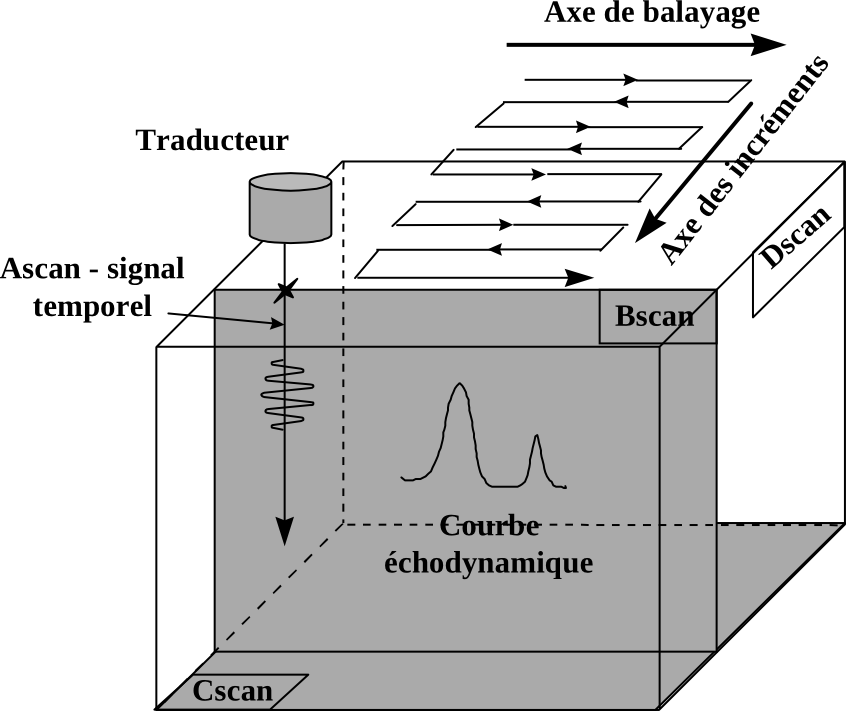
\includegraphics[scale=0.7]{img/scan.png}
%	\caption{\label{scan} Schéma des différents modes de représentation des signaux temporels (extrait de \cite{chassignole}).}
%\end{figure} 

\begin{figure}
	\centering
	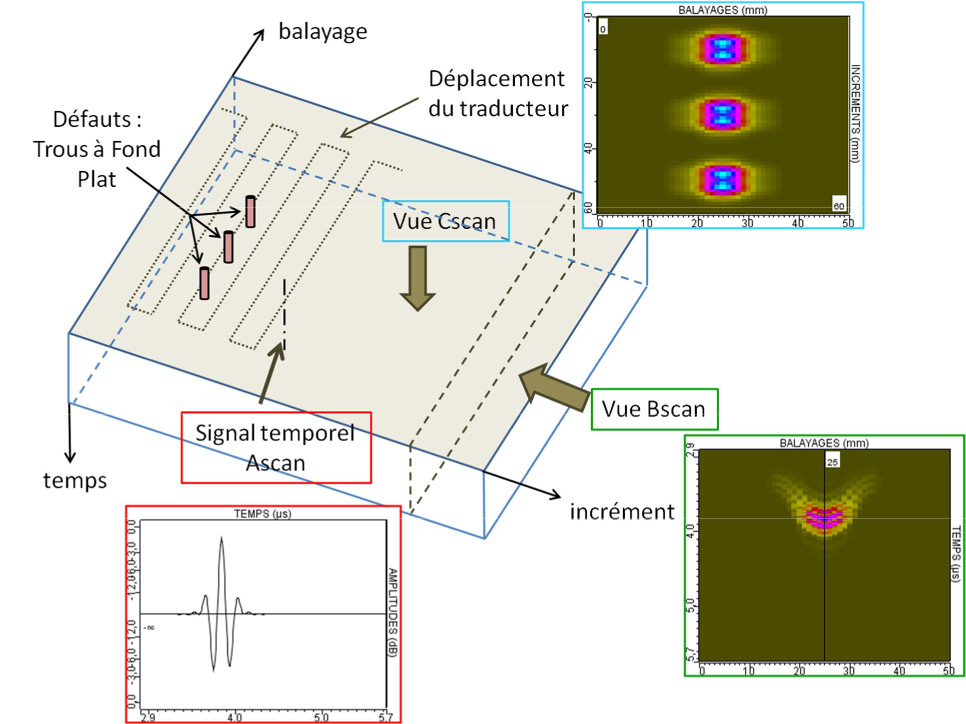
\includegraphics[scale=0.7]{img/scan2.png}
	\caption{\label{scan} Schéma des différents modes de représentation des signaux temporels (extrait de \cite{bannouf}).}
\end{figure}

En revanche, le Sscan ne peut être réalisé qu'avec des transducteurs multi-éléments. Il correspond a un ensemble de Ascans réalisés sans déplacement du transducteur mais en appliquant une loi de retard aux éléments permettant de réaliser un balayage du point focal. Le Sscan permet donc d'imager des pièces partiellement accessible, et augmente la probabilité de repérer un défaut en offrant plusieurs angles d'observation.\\

Cependant, la localisation dans la pièce des réflecteurs à l'origine des différents échos visibles sur les signaux temporels mesurés n'est possible que si la vitesse de propagation des ondes est connue. Les Bsans dits "vrais" sont des Bscans sur lesquels des corrections liées à la vitesse ou à l'angle d'incidence sont appliqués.


\section{Méthodes par retard et sommation}
Ces données temporelles peuvent aussi être post-traitées de manière à obtenir une représentation spatiale de la pièce. Si la vitesse du milieu de propagation est connue, une analyse des temps de vol des échos permet en effet d'établir une carte du milieu. \\

Il est aussi possible de sommer un ensemble de Ascans de façon cohérente, permettant ainsi de reproduire une focalisation en tous points de la zone à inspecter. C'est que proposent la méthode Synthetic Aperture Focusing Technique \citep{doctor_saft} à partir des signaux recueillis par un mono-éléments. Ce procédé est généralisé à un ensemble de capteurs et d'émetteurs dans la méthode Total Focusing Method \citep{holmes_tfm}. 

L'intensité $I$ de l'image obtenue au point de coordonnées $\bm{r}$ est alors donnée par la relation suivante : 

\begin{equation*}
	I(\bm{r})= \displaystyle\sum_{r} \displaystyle\sum_{t} s_{r,t}\left( \frac{|\bm{r} - \bm{r}_r| + |\bm{r} - \bm{r}_t|}{c}\right) \text{,}
\end{equation*}
où $\bm{r}_r$ et $\bm{r}_t$ sont les positions des récepteurs et des émetteurs, $s_{r,t}$ sont les signaux temporels pour chaque couple émetteur-récepteur et $c$ est la vitesse de l'onde dans le milieu de propagation.

Cette focalisation permet donc de couvrir l'ensemble du volume de la pièce car tous les angles peuvent être balayés, indépendamment de l'ouverture du capteur, ce qui permet une meilleure résolution que celle obtenue avec des Bscans.\\






\section{Méthodes hautes résolution}


Des méthodes de localisation de sources dites "hautes résolutions" exploitent l'ensemble des covariances des signaux temporels. Les méthodes telles que MUltiple Signal Classification \citep{schmidt} et Capon \citep{capon} proposent une décomposition en valeurs propres de cette matrice de covariance afin d'en extraire deux sous-espaces bruit et signal, diminuant ainsi la contribution énergétique du bruit. \\

La méthode de Décomposition de l'Opérateur de Retournement Temporel \citep{prada_2002} propose, de la même façon, d'interpréter l'opérateur de retournement temporel comme une matrice de covariance et de la décomposer. Cette dernière méthode est particulièrement adaptée aux milieux hétérogènes et/ou à géométrie complexe , puisqu'elle tire profit des réflexions multiples.  

Tous comme les méthode de formation de voies classiques, il est nécessaire de connaître les propriétés élastiques du milieu de propagation pour pouvoir localiser précisément les réflecteurs.\\

%(billette de titane, par exemple https://www.institut-langevin.espci.fr/IMG/pdf/jasakerbrat-2002.pdf)
%(plaque mince : ondes de lamb https://www.institut-langevin.espci.fr/IMG/pdf/JASAlamb-1998.pdf)

\section{Résolution de problème d'optimisation}

L'objectif de ces méthodes est de résoudre un problème inverse en minimisant une fonction coût traduisant l'écart entre le modèle calculé et le modèle vrai \citep{tarantola_book}. Le modèle est décrit par un nombre fini de paramètres $\bm{m}$ qui sont liés à des observables $\bm{d}_{obs}$ par l'intermédiaire de lois physiques $\bm{g}$. La résolution du problème inverse consiste donc à trouver les paramètres $\bm{m}$ optimaux à partir des données $\bm{d}_{obs}(\bm{m})$ (cf schéma de la figure~\ref{pb_inv}). 

\begin{figure}[!h]
	\centering
	\begin{tikzpicture}
		\node (param) [draw=black, align=center] at (0,0) {Paramètres initiaux \\ $\bm{m}_{0}$};
		\node (dir) [below=1cm of param , draw=black,align=center] {Problème direct \\ $\bm{g}(\bm{m})$};
		\path[->, thick,shorten <=2pt,shorten >=2pt] (param) edge (dir);
		\node (fc) [draw=black,right=2cm of dir, align=center] {Fonction de coût \\ $\text{écart}\hspace{-1mm}\left(\bm{d}_{obs}, \bm{d}_{cal}(\bm{m})\right)$};
		\path[->, thick,shorten <=2pt,shorten >=2pt] (dir) edge (fc);
		\node (m) [draw=black, below right= and -0.5cm of dir, align=center] {Problème inverse \\$\bm{m}+\Delta\bm{m}$};
		\path[->, thick,shorten <=2pt,shorten >=2pt] (fc) edge (m);
		\path[->, thick,shorten <=2pt,shorten >=2pt] (m) edge (dir);
	\end{tikzpicture} 
	\caption{\label{pb_inv} Schéma de résolution d'un problème d'optimisation.}
\end{figure}

Ces problèmes sont, en général, non-linéaires, car les observables ne dépendent pas linéairement des paramètres du modèle. De plus, si le nombre de paramètres est grand devant le nombre d'observables, ils sont également mal posés.\\

\subsection{Résolution du problème direct}

Le problème direct peut être résolu soit par des méthodes analytiques (représentation intégrale, méthodes modales,\ldots) soit par des méthodes numériques. Parmi les méthodes numériques les plus usitées figurent : les méthodes de différences finies (\citealp{virieux_86}, à l'ordre 2 et \citealp{levander}, à l'ordre 4), les méthodes des éléments finis (Galerkin discontinu par exemple : \citealp{brossier_these}) ou volumes finis \citep{brossier_2008}, les lancers de rayons \citep{virieux_ray}. 

\subsection{Résolution du problème inverse}
Si le problème direct possède une solution unique, ce n'est pas le cas du problème inverse.
Lorsque le nombre de paramètres est grand, le problème inverse ne peut pas être résolu par une recherche exhaustive dans l'espace des solutions. La recherche de solution peut donc se faire de manière semi-globale ou locale.\\

\subsubsection{Les méthodes semi-globales}
Les méthodes semi-globales consiste a parcourir l'espace des solutions avec une approche statistiques. Les plus connues sont les améliorations de celle de Monte Carlo comme le recuit simulé \citep{tarantola_book, sen} ou  la méthode de Monte-Carlo par chaînes de Markov \citep{zhang}, ainsi que les algorithmes génétiques. Elles permettent d'assurer une convergence avec peu d'\emph{a priori} sur le modèle initial.\\

\subsubsection{Les méthodes locales}
Lorsque que le modèle initial comporte suffisamment d'informations pour que le problème se situe proche du minimum global recherché, des méthodes d'optimisation moins coûteuses sont envisageables. Ces méthodes se basent sur l'estimation du gradient et du hessien de la fonction coût pour estimer sa plus forte pente et sa courbure.\\

La méthode de recherche linéaire la plus simple est celle du gradient (ou algorithme de la plus forte pente), qui permet d'effectuer au point courant, un pas de descente dans la direction opposée au gradient. Les directions de descentes successives sont alors orthogonales, ce qui ne permet pas une convergence très rapide. \\
La méthode du gradient conjugué propose de combiner les directions de descente des itérations précédentes de façon à accélérer la convergence. Cette méthode populaire est celle utilisée par Mora et Tarantola dans les années 80 \citep{tarantola_84, mora_87a, mora_87b}. Le hessien n'est pas calculé, mais cette méthode nécessite le calcul de deux problèmes directs supplémentaires. \\

Les méthodes full-Newton et Gauss-Newton utilisent le calcul du hessien (complet pour la première, approximé pour la seconde), ce qui permet une convergence plus rapide qu'avec la méthode du gradient conjugué, sans coût excessif supplémentaire \citep{pratt_98}.\\

Enfin, le hessien peut également être estimé à partir des gradients des itérations précédentes, par la méthode quasi-Newton \citep{nocedal}, avec l'algorithme BFGS (Broyden, Fletcher, Goldfarb, Shanno), par exemple. Cet algorithme ayant un gros coût de stockage, il existe des versions allégées fournissant une estimation du hessien à partir du stockage de quelques itérations seulement (L-BFGS). 
\subsection{Cartographie ou contour}
Comme le souligne les auteurs du chapitre 1.4 de BruneauPotel, le problème inverse peut être résolu suivant deux approches : 
\begin{itemize}
	\item un formalisme en intégrales de contour où les paramètres reconstruits sont ceux décrivant ces contours. Cela revient donc à déterminer la topologie d'un milieu. Le gradient, donné par la dérivée de la fonction coût par rapport à la topologie, indique donc directement la position d'un défaut à fort contraste. \cite{dominguez} et \cite{rodriguez} utilisent par exemple cette approche pour des applications en contrôle non destructif. Cette approche permet par exemple d'imager des défauts liés à une absence de matière (porosité, fissure, délaminage,\ldots) mais ne permet pas de caractériser des défauts de contraste plus faible (inclusion, corps étranger,\ldots).
	\item une reconstruction pixelisées d'un ensemble de paramètres. C'est l'approche adoptée pour la FWI et qui est décrite au chapitre~\ref{fwi}.
\end{itemize}


%-mais aussi : diffraction tomograhy, filtered backpropagation... : techniques basées sur une version linéarisée des équations, born approx par ex, kirchhoff approx


\section{Spécificités de l'imagerie de soudure}

Nombre de ces méthodes sont peu adaptées à l'imagerie de soudure. En effet, comme le montrent les macrographies de la figure~\ref{soudure}, les passes multiples et la cristallisation inhomogène rendent la soudure fortement anisotrope \citep{chassignole}. Cette anisotropie varie d'unes soudure à une autre puisqu'elle dépend des paramètres de soudage. En conséquence, cette anisotropie engendre une courbure voire une division du faisceau ultrasonore. Les scans sont alors difficiles à analyser (cf figure \ref{echos}), les méthodes par retard et sommation ne permettent pas de relocaliser précisément un réflecteur et les images obtenues sont très sujettes aux artefacts provenant d'échos mal interprétés.

\begin{figure}[!h]
	\hspace{-2cm}
    \centering
    \begin{subfigure}[c]{0.25\textwidth}
    	\centering
        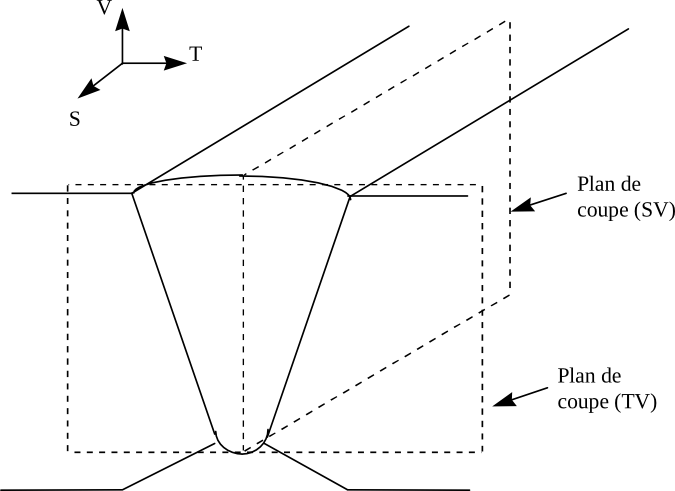
\includegraphics[height=3.5cm]{./img/soudure3.png}
        \vspace{0.03cm}
        \caption{\centering  Définition des plans de coupe.}
    \end{subfigure}
    \hspace{1cm}
    \begin{subfigure}[c]{0.25\textwidth}
    	\centering
        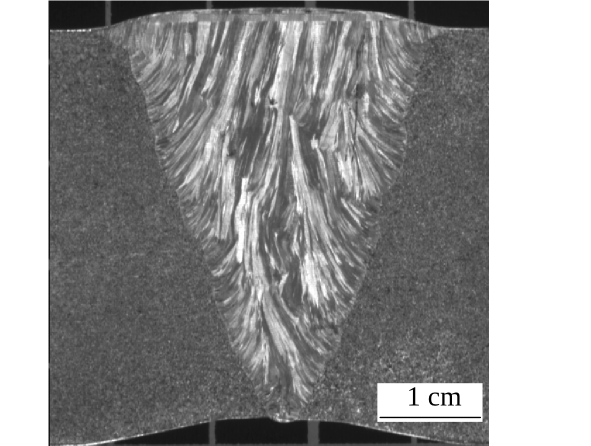
\includegraphics[height=4cm]{./img/soudure1.png}
        \caption{\centering  Coupe dans le plan (TV).}
    \end{subfigure}
        \hspace{1.5cm}
    \begin{subfigure}[c]{0.25\textwidth}
    	\centering
		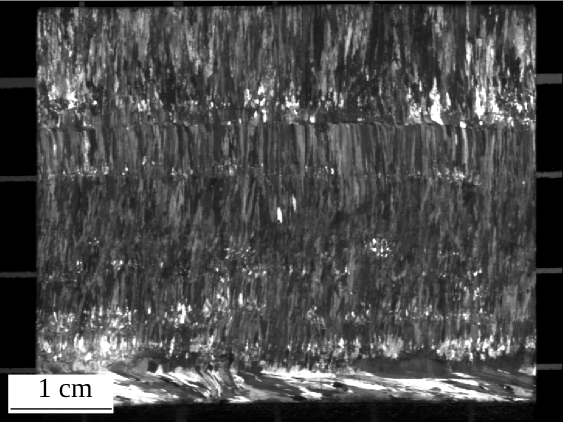
\includegraphics[height=4cm]{./img/soudure2.png}
        \caption{\centering Coupe dans le plan (SV).}
    \end{subfigure}
    \caption{Macrographie d'une soudure industrielle en acier inoxydable en acier austénitique \citep{chassignole}. À gauche : coupe dans le plan $(x,z)$, à droite : coupe dans le plan $(x,y)$.\label{soudure}}
\end{figure}

\begin{figure}[!h]
    \centering
    \begin{subfigure}[c]{0.3\textwidth}
    	\centering
        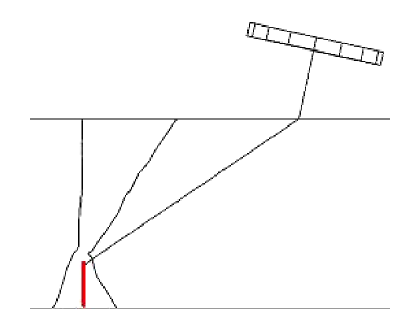
\includegraphics[height=4cm]{img/chassignole_echos_config.png}
        \caption{Configuration de mesure. En rouge : encoche de 15~mm de haut dans la soudure.}
    \end{subfigure}
    \hspace{1cm}
    \begin{subfigure}[c]{0.3\textwidth}
    	\centering
        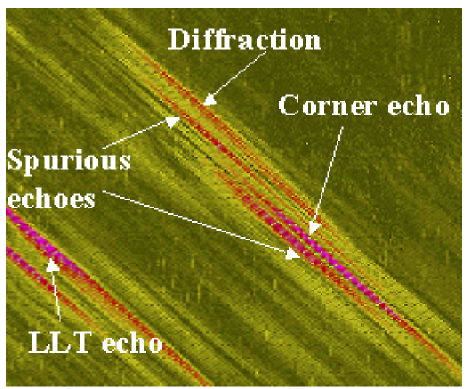
\includegraphics[height=4cm]{img/chassignole_echos.png}
        \caption{Bscan}
    \end{subfigure}
    \caption{Illustration de la perturbation du faisceau ultrasonore dans une sourdure. Images extraites de \cite{chassignole_beam}. LLT echo : Réflexion de l'onde longitudinale (L) sur le bord de soudure puis réflexion de cette onde L sur l'encoche avec conversion en mode transverse (T).  }\label{echos}
\end{figure}

De manière générale, les méthodes nécessitant une bonne connaissance du matériau ne sont pas adaptées à l'imagerie de soudure ; tenter de reconstruire les paramètres élastiques de la soudure par une résolution de problème inverse semble être une approche plus appropriée.




\todo[inline]{}

%hohne\_2012 pour images SAFT


%gardahaut pour porpagation de rai CIVA

%Born : linéarise le pb ? (pour faible contraste, adapté au cnd ?) brossier these dit que c'est pas linéarisé et qu'on a donc le champ d'onde complet

%+acoustique non-linéaire : Nonlinear signal processing for ultrasonic imaging of material complexity (dos santos) par ex
